\chapter{Experimental method}

\paragraph{}
This section describes the experimental method used to assess the performance of the state-decomposition method. This is done by
implementing different versions of the state-decomposition method, testing them in different environments and
comparing the performance with a baseline algorithm. 

\section{Tools}

\paragraph{Python}
The programming language chosen for this project is Python. This is motivated by Python being a high-level language that allows
writing compact, readable code and by the widespread availability of resources and packages for it. Additionally, Python can be
run on Colab notebooks, which are described in the next paragraph.

\paragraph{Google Colaboratory (Colab)}
Colab is a platform from Google which is widely used for machine learning research and prototyping of new models. Colab combines a
notebook platform that many Python developers are familiar with and the high-performance of cloud computing. The user can choose
to run a program using CPUs, GPUs, or TPUs\footnote{Tensor Processing Unit: a custom hardware accelerator developed by Google to
accelerate the linear algebra operations that occur in machine learning. \cite{noauthor_cloud_nodate}}. Examples of the available
GPUs are Nvidia K80 and NVidia P100D. The disadvantage of Colab compared to cloud computing platforms such as Google Cloud and
Amazon AWS is that the user is not guaranteed full access to the hardware accelerators (such as GPUs) and thus the performance can
vary. The session length is also limited to 12 hours. These problems are mitigated by purchasing a "Pro" license for the price of
\$10 per month, which prioritises access to GPUs and increases the maximum session length to 24 hours. The main advantage is an
easy to use platform thanks to its notebook format which allows for easy prototyping, rather than the less user-friendly access
via SSH in the Terminal required by other cloud-computing platforms. 

\paragraph{Keras}
In this work the deep-learning models are implemented using the deep-learning API Keras \cite{keras}. This is a high-level
interface that uses Tensorflow \cite{noauthor_tensorflow_nodate} for its backend. Keras allows to code deep-learning models in a
very readable and compact way. Having Tensorflow as its backend, it can run on CPUs, GPUs, and TPUs, taking advantage of the
high-performance hardware offered by Google Colab.

\paragraph{OpenAI Gym}
As this project deals with the development and evaluation of a new method for reinforcement learning algorithms, it is decided to
apply it in a "toy environment" that would simplify experimentation and provide insight into how the decomposition techniques
would operate. OpenAI offers an open-source Python toolkit called "OpenAI Gym" \cite{openai_gym_nodate}, which is currently the
most commonly used toolkit to benchmark reinforcement learning algorithms. This toolkit offers a variety of different
environments, ranging from classical control problems such as "CartPole-v0" \cite{noauthor_openai_nodate}, to more complicated
environments such as playing Atari games using the pixel data as sensory input or solving robotic manipulation problems. The
"OpenAI Gym" offers environments with a wide range of complexities and all combinations of discrete and continuous state and
action spaces. Figure \ref{fig:cartpole} shows a screenshot of one of the most popular environments in the toolkit.

\begin{figure}[H]
    \centering
    \includegraphics[width = 0.5\linewidth]{figures/cartpole.PNG}
    \caption{The CartPole-v1 environment is one of the most well-known environments of the OpenAI Gym library in which the goal is
    to balance the cartpole while keeping it within the boundaries of the screen by applying a leftwards or a rightwards force at
    each time-step. Screenshot of \cite{noauthor_openai_nodate}.}
    \label{fig:cartpole}
\end{figure}

\section{Testing environments} \label{sec:TaxiTraps}

\paragraph{}
The state-transition matrices and their decomposed versions were obtained\footnote{These were obtained by "cheating" by simply
inspecting the source code of the environments.} for 4 different OpenAI Gym environments: "Cartpole-v1"\footnote{This environment
has continuous states which are discretised using a linear quantiser to apply the decomposition algorithm.}, "FrozenLake8x8-v0",
"CliffWalking-v0" and "Taxi-v3". The state decomposition algorithm is aimed at environments whose state-spaces decompose into
similarly sized sub-spaces, as this is the case in which the method would be potentially very effective. If one of the
state-spaces is much greater than the others and similar in size to the original state-space, the reduction in complexity of
training an agent for this sub-space would not be as significant. Having sub-spaces that are too small (in the extreme case having
just one state) limits the amount of learning that can be achieved by the sub-spaces' agents, so that learning to combine the
sub-agents could be very complex and slow. The MDPs of "Cartpole-v1", "FrozenLake8x8-v0" and "CliffWalking-v0" don't decompose into
similarly sized sub-spaces, thus they are not suitable for testing the state decomposition method.

\paragraph{}
The "Taxi-v3" environment, shown on the left in Figure \ref{fig:taxi} has then been deemed to be a more suitable candidate. The
environment has:
\begin{itemize}
    \item 500 discrete spaces, corresponding to 25 taxi positions in the 5x5 grid, 4 possible destinations, and 5 possible
    passenger positions (1 of which is inside the taxi).
    \item 6 discrete actions: 4 moves (up, down, left, right), pick-up passenger, and drop-off passenger.
    \item Rewards: +20 for a successful drop-off, -1 at each time step (also when hitting a wall), and -10 for illegal pick-up and
    drop-off actions.
\end{itemize}

An episode terminates when the passenger is successfully dropped off or after 200 time-steps. Applying the state decomposition to
this environment can form 4 equally sized sub-spaces even with a threshold of 0, meaning that these are 4 completely independent
sub-spaces that can be treated as independent Markov Decision Processes. These 4 sub-spaces correspond to the 4 possible
destinations of the passenger, which never change during a single episode. Thus, this is a more specific and easier problem than
the one we are trying to solve, where the subsystems, though rarely, do interact with each other. 

\paragraph{}
This project then proposes a modified version called "TaxiTraps", shown in the middle in Figure \ref{fig:taxi}, in which the
transition probabilities were modified to allow a small amount of interaction between sub-spaces\footnote{Making transition
probabilities between spaces of different subsystems non-zero.} in order to test in the more general case. This has added "traps"
located on the edges of certain cells of the grid. These activate with a low probability $p_{trap}$ when the Taxi moves over them.
If a trap does not activate, the taxi simply moves over it as in the original "Taxi-v3" environment. When the trap does activate,
the behaviour of the environment is modified in two ways:

\begin{enumerate}
    \item The destination of the Taxi changes, thus transitioning to a different sub-space.
    
    \item The agent receives a highly negative reward. This is added to ensure that the optimal policy in the "TaxiTraps" environment is
    different than in the original Taxi environment. Since in the first stage of the original state decomposition method the transitions
    between different state sub-spaces are ignored, the agents are trained in an environment equivalent to the original "Taxi-v3".
    If the optimal policy is the same in "Taxi-v3" and "TaxiTraps", the optimal policy would not change between the first and
    second training stage of training, which is unlikely to happen in a general scenario. Thus, ensuring that the optimal policy
    changes between training stages is required for the results of testing to generalise to other environments.  
\end{enumerate}

\paragraph{}
During testing it has been noted that the two 'Taxi' environments would take a very high number of iterations to train and would
often get stuck for long periods of time at reward -200, which is when the agent has learned to not commit illegal moves but it
has not learned to drop-off the passenger successfully. Due to the limited computing power of my tools, this is a problem as it
does not allow for significant testing with a high number of trials. Thus, it has been decided to try using a simpler version of
the 'Taxi' environment, called 'Taxi2', shown on the right in Figure \ref{fig:taxi}. The number of destinationations is reduced to
2 and the multi-stage nature of the task, having to pick-up the passenger, navigate the grid and then drop it off, is eliminated
by setting the passenger to always be inside the Taxi, so that the pick-up and drop-off actions are eliminated and the task is
completed by simply reaching the destination. 

\begin{figure}[H]
\centering
    \resizebox{\linewidth}{!}{
    \subfloat["Taxi"]{
        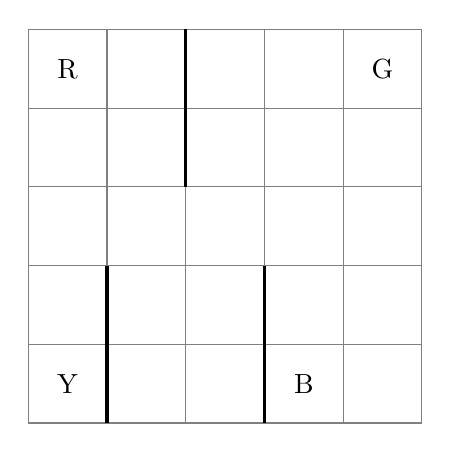
\begin{tikzpicture}
            \draw[step=1cm,color=gray] (0,0) grid (5,5);
            \node at (0.5,4.5) {R};
            \node at (4.5,4.5) {G};
            \node at (0.5,0.5) {Y};
            \node at (3.5,0.5) {B};
            \draw[very thick] (2,5) -- (2,3);
            \draw[very thick] (1,2) -- (1,0);
            \draw[very thick] (3,2) -- (3,0);
        \end{tikzpicture}}
    \qquad
    \subfloat["TaxiTraps"]{
        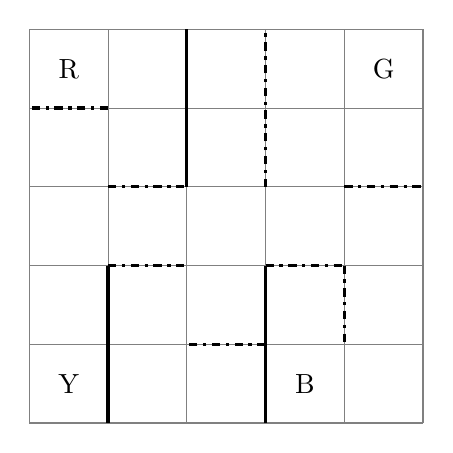
\begin{tikzpicture}
            \draw[step=1cm,color=gray] (0,0) grid (5,5);
            \node at (0.5,4.5) {R};
            \node at (4.5,4.5) {G};
            \node at (0.5,0.5) {Y};
            \node at (3.5,0.5) {B};
            \draw[very thick] (2,5) -- (2,3);
            \draw[very thick] (1,2) -- (1,0);
            \draw[very thick] (3,2) -- (3,0);
            \draw[very thick, dash dot] (1,4) -- (0,4);
            \draw[very thick, dash dot] (1,3) -- (2,3);
            \draw[very thick, dash dot] (3,1) -- (2,1);
            \draw[very thick, dash dot] (1,2) -- (2,2);
            \draw[very thick, dash dot] (3,2) -- (4,2);
            \draw[very thick, dash dot] (4,3) -- (5,3);
            \draw[very thick, dash dot] (3,3) -- (3,5);
            \draw[very thick, dash dot] (4,2) -- (4,1);
        \end{tikzpicture}}
    \qquad
    \subfloat["Taxi2"]{
        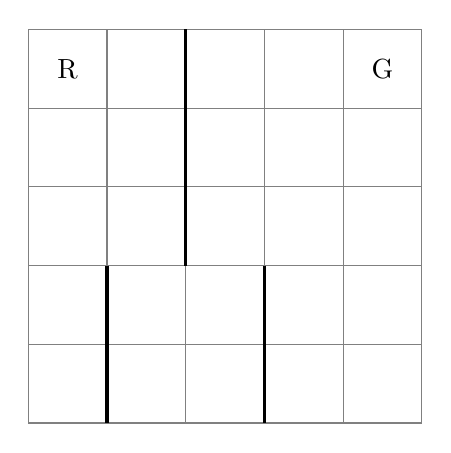
\begin{tikzpicture}
            \draw[step=1cm,color=gray] (0,0) grid (5,5);
            \node at (0.5,4.5) {R};
            \node at (4.5,4.5) {G};
            \draw[very thick] (2,5) -- (2,3);
            \draw[very thick] (1,2) -- (1,0);
            \draw[very thick] (3,2) -- (3,0);
            \draw[very thick] (2,3) -- (2,2);
        \end{tikzpicture}}}
    \caption{Original and modified 'Taxi' environments. The thick black lines represent the walls, while the dotted lines represent the "traps".}
    \label{fig:taxi}
\end{figure}

\paragraph{}
While 'Taxi2' reduces the complexity of training, this was still not simple enough and it didn't allow for easy interpretability
of the results. I then introduced the 'Grid' environment, which is a simple 25 by 25 grid with two destinations, as shown in
Figure \ref{fig:grid}. Those positions in the grid on the upper-left side of the dotted line in the figure are referred to as the
'upper-left triangle' or 'triangle 1', while those on the lower-right side are the 'lower-right triangle' or 'triangle 2'. At the
start of the episode, the taxi is initialised in a random position, while the passenger is always assumed to be inside the Taxi,
as in 'Taxi2', so that the pick-up and drop-off actions are eliminated and the learning process only deals with learning how to
navigate in the grid. The two destinations are located at opposite corners and the initial destination is always chosen to be the
one closest to the initial position of the taxi. 'Destination 1' is at the upper-left corner and 'destination 2' is at the
bottom-right corner. Throughout an episode the destination always remains the same as in the initial state and the episode
terminates when the taxi reaches the correct destination. To summarise, the environment has:
\begin{itemize}
    \item 1250 discrete states, corresponding to 625 taxi positions in the 25x25 grid and 2 possible destinations.
    \item 4 discrete actions: move up, down, left and right.
    \item Rewards: +20 for being in the position chosen as the destination, -1 at each time step (also when hitting a boundary and
    thus not moving).
\end{itemize}

\begin{figure}[H]
    \centering
    \resizebox{0.5\linewidth}{!}{
    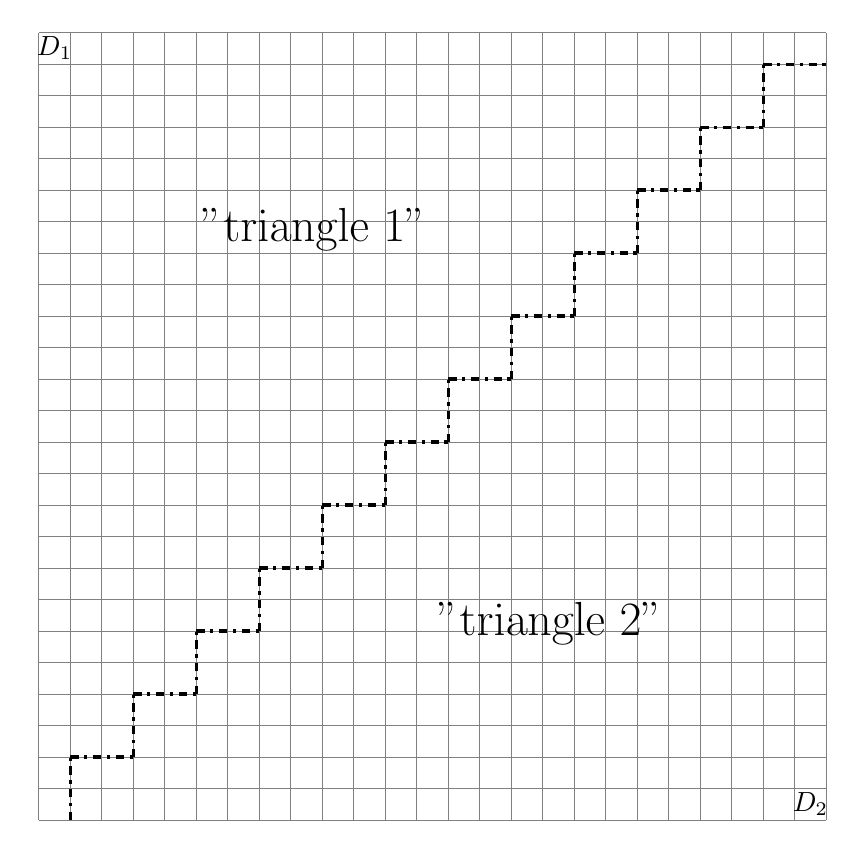
\begin{tikzpicture}
        \draw[step=0.4cm,color=gray] (0,0) grid (10,10);
        \node at (0.2,9.8) {$D_1$};
        \node at (9.8,0.2) {$D_2$};
        \node at (3.5,7.5) {\LARGE "triangle 1"};
        \node at (6.5,2.5) {\LARGE "triangle 2"};
        \draw[very thick, dash dot] (9.2,9.6) -- (10.0,9.6);
        \draw[very thick, dash dot] (9.2,8.8) -- (9.2,9.6);
        \draw[very thick, dash dot] (8.4,8.8) -- (9.2,8.8);
        \draw[very thick, dash dot] (8.4,8.0) -- (8.4,8.8);
        \draw[very thick, dash dot] (7.6,8.0) -- (8.4,8.0);
        \draw[very thick, dash dot] (7.6,7.2) -- (7.6,8.0);
        \draw[very thick, dash dot] (6.8,7.2) -- (7.6,7.2);
        \draw[very thick, dash dot] (6.8,6.4) -- (6.8,7.2);
        \draw[very thick, dash dot] (6.0,6.4) -- (6.8,6.4);
        \draw[very thick, dash dot] (6.0,5.6) -- (6.0,6.4);
        \draw[very thick, dash dot] (5.2,5.6) -- (6.0,5.6);
        \draw[very thick, dash dot] (5.2,4.8) -- (5.2,5.6);
        \draw[very thick, dash dot] (4.4,4.8) -- (5.2,4.8);
        \draw[very thick, dash dot] (4.4,4.0) -- (4.4,4.8);
        \draw[very thick, dash dot] (3.6,4.0) -- (4.4,4.0);
        \draw[very thick, dash dot] (3.6,3.2) -- (3.6,4.0);
        \draw[very thick, dash dot] (2.8,3.2) -- (3.6,3.2);
        \draw[very thick, dash dot] (2.8,2.4) -- (2.8,3.2);
        \draw[very thick, dash dot] (2.0,2.4) -- (2.8,2.4);
        \draw[very thick, dash dot] (2.0,1.6) -- (2.0,2.4);
        \draw[very thick, dash dot] (1.2,1.6) -- (2.0,1.6);
        \draw[very thick, dash dot] (1.2,0.8) -- (1.2,1.6);
        \draw[very thick, dash dot] (0.4,0.8) -- (1.2,0.8);
        \draw[very thick, dash dot] (0.4,0.0) -- (0.4,0.8);
    \end{tikzpicture}}
    \caption{'Grid' environment. The dotted lines have no effect on the environment, they simply separate the grid positions part of 'triangle 1' and 'triangle 2'.}
    \label{fig:grid}
\end{figure}

\paragraph{}
This is a perfectly decomposable environment, as there are no possible transitions between states having different destinations.
For a complete evaluation of the state-decomposition method, it needs to be tested in a more generic environment, with non-zero
albeit small transition probabilities between the decomposed sub-spaces. This is achieved by introducing a probability $\epsilon$
of changing the destination whenever the current destination is the one closest to the current position in the grid. The initial
destination can now be the far one, with probability $\epsilon$. This modified 'Grid' environment will be referred to as
'GridEps'. Table-\ref{table:state-transitions-GridEps} summarises the transition probabilities in 'GridEps'.

\begin{table}[H]
    \centering
    \begin{tabular}{cl|ll|}
    \cline{3-4}
    \multicolumn{1}{l}{}                         &                            & \multicolumn{2}{c|}{next state}                                \\ \cline{3-4} 
    \multicolumn{1}{l}{}                         &                            & \multicolumn{1}{l|}{destination 1} & destination 2             \\ \hline
    \multicolumn{1}{|c|}{\multirow{4}{*}{state}} & triangle 1 - destination 1 & $1-\epsilon$          & $\epsilon$                  \\
    \multicolumn{1}{|c|}{}                       & triangle 1 - destination 2 & 0                                  & 1                         \\
    \multicolumn{1}{|c|}{}                       & triangle 2 - destination 1 & 1                                  & 0                         \\
    \multicolumn{1}{|c|}{}                       & triangle 2 - destination 2 & $\epsilon$           & $1-\epsilon$ \\ \hline
    \end{tabular}
    
    \caption{State transition probabilities in the 'GridEps' environment.}
    \label{table:state-transitions-GridEps}
\end{table}

\paragraph{}
The transition probabilities are chosen in this way to achieve the following effects. That is, while providing small transition
probabilities between different sub-spaces, changes in $\epsilon$ also change the optimal policy. This is important as
the case in which the optimal policy is unaffected by the value of $\epsilon$ is a special case which should not be used for
testing.

\paragraph{}
Another version that is used in various testings is very similar to 'GridEps' and will be called 'GridEps2'. The difference is in
the probabilities with which the destination is picked in each time-step. In this case, when the current destination is the closer
one betweeen the two possible destinations, the destination in the next state is the closer destination to the position in the
next state with probability $1-\epsilon$ and the other one with probability $\epsilon$, whereas in 'GridEps' the destination in
the next state depends on the position of the current state. This only makes a difference in transitions that cross the boundary
between the two "triangles". In 'GridEps', when the boundary is crossed and the destination was the close one, the destination
most likely remains the same, while in 'GridEps2' it most likely switches to the other one, which is the closest after crossing
the boundary. This may seem like a small difference, but it has a significant impact on the effect of how the states are
decomposed, as mentione in the next chapter.

%Is the fact that we are discouraging the Taxi to go over the traps a problem as in the final policy we are kind of ignoring
%transitions because we actively avoid them?

\paragraph{}
'GridEps' is an example of a scenario in which the decomposition is "intuitive", as mentioned in
Section \ref{sec:decomposing-trans-matrix}. It is clear here that one possible decomposition is given by creating one sub-space
for each possible destination, as at each-time the probability of changing destination is very small, being either $0$ or
$\epsilon$. Another kind of decomposition that has been tested, although it does not necessarily follow the procedure previously
described for decomposing the state-transition matrix for $\epsilon > 0$, is to assign states corresponding to positions in the
upper-left "triangle" of the grid to one sub-space and positions in the lower-right "triangle" to the other sub-space. The reasoning
is that when $\epsilon$ is 0, following the optimal policy would lead to never crossing the boundary between these two
"triangles", meaning that they form two independent sub-spaces. When $\epsilon > 0$, this can happen and the transitions between
the two sub-spaces are not small, thus it is an interesting example of using a different kind of decomposition that is not based
on single transition probabilities.

\paragraph{}
It is possible to use policy iteration to determine the optimal policy and the optimal state values as we have access to the
models' dynamics. This is used to make sure that the tested reinforcement learning algorithms, which are model-free, as they are
not given the dynamics of the model as input, actually perform optimal actions and reach convergence after enough training. 

\section{Benchmark DQN agent}

\paragraph{}
The aim of this project is to determine whether state decomposition techniques can be used to increase the sample efficiency of
reinforcement learning algorithms. Doing so requires comparing the performance of an algorithm where state decomposition is
applied and that of an equivalent algorithm without state decomposition, while choosing all other parameters to be the same or to
be the values that make for the fairest comparison. The number of possible choices to be made in these algorithms is such that
providing a fair comparison can be a non-trivial task, as discussed in Section \ref{sec:fair-comparison}. 

\paragraph{}
The chosen benchmark RL agent is a basic DQN agent. The value updates occur with discount factor $\gamma=0.95$. It would be
possible to use $\gamma=1$, as the algorithm in tested in environments with finite length episodes, however, using a slightly
smaller discount factor enhances the stability of the algorithm, giving more consistent results. The agent acts according to an
$\epsilon$-greedy policy. This involves a parameter called $\epsilon$ that is a different parameter and unrelated to the
$\epsilon$ that represents the probability of transitions between different sub-spaces in 'GridEps'. This means that at each
agent-environment interaction, the agent picks the action that currently has the highest estimated action value with probability
$1-\epsilon$ or a random action with probability $\epsilon$. $\epsilon$ is initialised at 1, meaning that in the first iteration
the action is completely random. $\epsilon$ decays by a factor $0.999$ after each update of the action values. $\epsilon$ is set
to stop decreasing at $\epsilon=0.01$, this is to ensure that the algorithm does not stop exploring by having too small an
$\epsilon$. 

\paragraph{}
Figure \ref{fig:DQN-network} shows the neural network that approximates the Q-values, which is fully connected and has 4 layers.
The input state is fed as an integer to an encoding layer\footnote{This is fixed and pre-programmed and does not include any
learned parameters.}, which then feeds to the first fully-connected layer, consisting of 512 neurons with "ReLU"\footnote{"ReLU"
stands for Rectified Linear Unit. It represents the function $f(x)=\max(0, x)$.} activation function. This is then followed by 2
similar layers, having 256 neurons each. The last layer consists of a number of neurons corresponding to the number of actions in
the environment where the agent is being used. Each output of the network corresponds to an action value of the input state, thus
the activation function in the last layer is an identity function. This is to allow the outputs to take any possible values,
without upper or lower bounds so that the network is theoretically capable of mapping any state to any possible
action value\footnote{Contrarily to for example a "ReLU" activation function, which wouldn't allow to have negative outputs}. The
network is updated using "Minimum Square Error" as its loss function, that is, at each update step, the network weights are
updated to reduce the function $L = \sum_{i=1}^n (y_i-f_{\theta}(x_i))^2$ where $x_i$ are the inputs, $y_i$ the corresponding
outputs and $f_{\theta}$ is the function implemented by the neural network with weights $\theta$. The network updates are done
using the optimiser Adam \cite{kingma_adam_2017}, a commonly used optimiser that achieves better performance than gradient descent
in many applications through the use of moments.

\begin{figure}[H]
    \centering
    \includegraphics[width = 0.8\linewidth]{figures/DQN.pdf}
    \caption{The neural network used for Q-values approximation in the baseline DQN algorithm.}
    \label{fig:DQN-network}
\end{figure}

\paragraph{}
Each iteration with the environment is saved in a replay memory as a $\langle S,A,R,S' \rangle$ tuple. The maximum size of this is
set to be big enough so that all samples are saved, without having to discard them in the later stages of training. After each
interaction with the environment, one update step of the neural network is run using a batch of 128 samples, randomly picked from
the replay memory.

\section{Ensuring fair comparison} \label{sec:fair-comparison}

When comparing the performance obtained using the state-decomposition technique with a benchmark method that does not use it, we
would like ideally to isolate the effect of the state-decomposition effect, independent to other changes to other parameters.
Unfortunately, it is not possible to perfectly isolate this effect, due to the complexity of the relationship between various
hyperparameters. However, it is possible to make reasonable choices such that the comparison is as fair as possible. In this
project, all hyperparameters are kept constant in all trials. Different experiments that involve different network architectures,
such as using 2 neural networks instead of 1 always ensure that the total number of trainable parameters in the neural networks of
each global agent is approximately equal. Other factors such as the encoding method of the state are always kept equal.
